\documentclass[11pt,letterpaper]{article}

\usepackage[margin=1in]{geometry}
\usepackage{setspace}
\onehalfspacing

\usepackage{microtype}
\usepackage{booktabs}
\usepackage{longtable}
\usepackage{array}
\usepackage{tabularx}
\usepackage{xcolor}
\usepackage{amsmath,amssymb}
\usepackage{tikz}
\usetikzlibrary{shapes.geometric, arrows.meta, positioning, fit, backgrounds}
\usepackage[hyphens]{url}
\usepackage[colorlinks=true,linkcolor=blue,citecolor=blue,urlcolor=blue]{hyperref}
\usepackage{cleveref}
\usepackage[numbers,sort&compress]{natbib}
\usepackage{enumitem}

\title{
    \vspace{-1cm}
    \textbf{Update 14: Kokkos Remote Spaces for GPU-Direct RDMA} \\[0.5em]
    \large PGAS-Based Distributed Shared Memory with GPUDirect and SR-IOV Testing
}

\author{
    Nathan Gopee \\
    \textit{MS Computer Science Candidate} \\
    SUNY New Paltz \\
    \texttt{gopeen1@newpaltz.edu}
}

\date{February 2026}

\begin{document}

\maketitle

\begin{abstract}
\noindent
This update investigates Kokkos Remote Spaces~\cite{kokkos-rs} as a Partitioned Global Address Space (PGAS) framework for distributed GPU memory access, with the goal of enabling GPUDirect RDMA across the heterogeneous lab cluster (RTX~3090, RTX~5090, Tesla~V100). We evaluate Kokkos Remote Spaces' four backends (SHMEM, NVSHMEM, ROCSHMEM, MPI one-sided), detail the GPUDirect RDMA setup process including \texttt{nvidia-peermem} and BAR1 memory configuration, and explore SR-IOV (Single Root I/O Virtualization) for RDMA NIC sharing in the Proxmox-hosted V100 environment. Additionally, we evaluate UCX (Unified Communication X)~\cite{ucx} as the transport abstraction layer, testing its \texttt{rc\_mlx5}, \texttt{gdr\_copy}, and \texttt{cuda\_ipc} transports across the cluster's heterogeneous NIC and GPU hardware. The analysis identifies which hardware configurations support true GPU-initiated RDMA and which require host-staged fallback paths.
\end{abstract}

%=============================================================================
\section{Kokkos Remote Spaces Overview}
%=============================================================================

Kokkos Remote Spaces~\cite{kokkos-rs} extends the Kokkos C++ performance portability framework~\cite{kokkos} with distributed shared memory (DSM) semantics. Rather than explicit MPI \texttt{Send}/\texttt{Recv} pairs, programmers allocate Kokkos Views in a \texttt{DefaultRemoteMemorySpace} that spans multiple processes and GPUs. Remote element access is handled transparently through one-sided RDMA operations---the accessing process does not require cooperation from the owning process.

\subsection{PGAS Programming Model}

In the PGAS model, a global address space is partitioned across processing elements (PEs). Each PE owns a contiguous segment, but any PE can read or write any location. Local accesses are fast (standard memory load/store); remote accesses incur network latency but require no explicit message passing. This maps naturally to GPU clusters: each GPU's memory is a partition, and remote accesses trigger RDMA operations.

Kokkos Remote Spaces distributes views by the left-most dimension. For a view of size $N$ across $P$ PEs, each PE owns $\lfloor N/P \rfloor$ rows. Global indexing automatically resolves the target PE and local offset:

\begin{equation}
    \text{PE} = \lfloor i / (\lfloor N/P \rfloor) \rfloor, \quad \text{offset} = i \bmod \lfloor N/P \rfloor
    \label{eq:pgas-mapping}
\end{equation}

\subsection{Backend Architecture}

Kokkos Remote Spaces supports four PGAS backends:

\begin{table}[htbp]
\centering
\caption{Kokkos Remote Spaces backend comparison}
\label{tab:backends}
\begin{tabular}{@{}lllll@{}}
\toprule
\textbf{Backend} & \textbf{GPU Support} & \textbf{Communication} & \textbf{Best For} & \textbf{Our Hardware} \\
\midrule
SHMEM & Host only & OpenSHMEM & CPU clusters & Fallback \\
NVSHMEM & CUDA (GPU-initiated) & GPUDirect RDMA & NVIDIA multi-GPU & V100 (Tower 2) \\
ROCSHMEM & HIP (GPU-initiated) & ROCm RDMA & AMD GPUs & N/A \\
MPI one-sided & Host only & \texttt{MPI\_Put}/\texttt{MPI\_Get} & Portable & All nodes \\
\bottomrule
\end{tabular}
\end{table}

The NVSHMEM backend is the most relevant for our cluster. It enables \textbf{GPU-initiated communication}: CUDA kernels can issue remote memory operations directly without returning to the host CPU. This eliminates the host-staging latency that plagues CPU-mediated RDMA approaches.

\subsection{Key APIs}

The core API extends Kokkos Views with remote memory semantics:

\begin{itemize}[noitemsep]
    \item \textbf{\texttt{DefaultRemoteMemorySpace}}: Memory space type for globally distributed allocations. Backed by \texttt{nvshmem\_malloc} (NVSHMEM), \texttt{shmem\_malloc} (SHMEM), or \texttt{MPI\_Win\_create} (MPI).
    \item \textbf{\texttt{PartitionedLayout}}: Layout policy distributing the left-most dimension across PEs.
    \item \textbf{\texttt{deep\_copy(local, remote)}}: Bulk transfer between local and remote views, mapped to \texttt{nvshmem\_putmem}/\texttt{nvshmem\_getmem} for NVSHMEM.
    \item \textbf{\texttt{local\_deep\_copy}}: Copies only the local PE's partition, useful for initialization.
    \item \textbf{\texttt{get\_local\_range(view)}}: Returns the index range owned by the calling PE.
    \item \textbf{\texttt{fence()}}: Ensures all remote operations from this PE have completed.
\end{itemize}

\subsection{Included Benchmarks}

The repository includes six benchmarks: \texttt{randomaccess} (GUPS---fine-grained random remote access), \texttt{stream} (sustained remote memory bandwidth), \texttt{access\_overhead} (per-access latency measurement), \texttt{misslatency} (remote miss penalty), \texttt{poissonaccess} (Poisson-distributed access patterns), and five applications: \texttt{cgsolve} (conjugate gradient with halo exchange), \texttt{heat3d} (3D heat equation stencil), \texttt{matvec} (distributed matrix-vector product), and \texttt{vectorshift} (cyclic vector permutation).

Performance data from Lassen (IBM Power9 + V100) shows that NVLink-connected GPU pairs achieve near-local bandwidth, while cross-socket accesses drop by ${\sim}4\times$---motivating the need for bulk transfer optimization via \texttt{deep\_copy} rather than fine-grained scalar access.

%=============================================================================
\section{GPUDirect RDMA: Architecture and Setup}
\label{sec:gpudirect}
%=============================================================================

GPUDirect RDMA enables a network interface card (NIC) to read from and write to GPU memory directly, bypassing the host CPU and system memory entirely. The data path is: GPU Memory $\to$ PCIe $\to$ NIC $\to$ Network $\to$ Remote NIC $\to$ PCIe $\to$ Remote GPU Memory.

\subsection{Required Components}

\begin{enumerate}[noitemsep]
    \item \textbf{\texttt{nvidia-peermem} kernel module}: Registers GPU BAR1 memory with the InfiniBand/RDMA subsystem. Loaded via \texttt{modprobe nvidia-peermem}. Replaces the deprecated \texttt{nv\_peer\_mem} module. Available in NVIDIA driver $\geq$470.
    \item \textbf{BAR1 memory}: The GPU's PCIe Base Address Register 1 maps GPU memory to the PCIe address space for DMA by external devices. Datacenter GPUs (V100, A100, H100) expose 16--256~GB BAR1; consumer GPUs (RTX 3090, 5090) expose only 256~MB by default.
    \item \textbf{RDMA-capable NIC}: InfiniBand or RoCEv2 NIC with OFED/rdma-core drivers. Mellanox ConnectX-4 (100~GbE) is the target NIC for both towers.
    \item \textbf{IOMMU configuration}: For GPUDirect RDMA to work, the GPU and NIC must be in the same IOMMU group or ACS (Access Control Services) must be disabled to allow peer-to-peer DMA across PCIe switches.
\end{enumerate}

\subsection{Consumer vs.\ Datacenter GPU Limitations}

\begin{table}[htbp]
\centering
\caption{GPUDirect RDMA capability by GPU class}
\label{tab:gpudirect-caps}
\begin{tabular}{@{}lcccc@{}}
\toprule
\textbf{GPU} & \textbf{BAR1 Size} & \textbf{nvidia-peermem} & \textbf{GPUDirect RDMA} & \textbf{Notes} \\
\midrule
Tesla V100 32GB & 32 GB & Supported & Full & Datacenter, Tower 2 \\
RTX 3090 24GB & 256 MB & Limited & Partial & Consumer, Chimera \\
RTX 5090 32GB & 256 MB & Limited & Partial & Consumer, Cerberus \\
RTX 5070 Ti 16GB & 256 MB & Limited & Partial & Consumer, Tower 1 \\
\bottomrule
\end{tabular}
\end{table}

The 256~MB BAR1 limitation on consumer GPUs means that only a small fraction of GPU memory is addressable via DMA. For a 24~GB RTX 3090, only 1\% of memory is BAR1-mapped. Large tensor transfers ($>$256~MB) must be staged through host pinned memory, negating the zero-copy benefit of GPUDirect.

\paragraph{Resizable BAR (ReBAR).}
Modern motherboards support Resizable BAR, which can expose the full GPU memory through BAR1. When enabled in BIOS, an RTX 3090 can expose all 24~GB through BAR1, enabling full GPUDirect RDMA. However, ReBAR support varies by motherboard vendor and may conflict with Above 4G Decoding settings.

\subsection{Setup Procedure for Tower 2 (V100 + ConnectX-4)}

The V100 on Tower~2 (Proxmox host) is the primary GPUDirect RDMA target. The setup sequence is:

\begin{enumerate}[noitemsep]
    \item Load the \texttt{nvidia-peermem} module: \texttt{modprobe nvidia-peermem}
    \item Verify registration in kernel log: \texttt{dmesg | grep peermem} should show ``nvidia peermem registered successfully''
    \item Confirm BAR1 availability: \texttt{nvidia-smi -q | grep BAR1} should report 32768~MiB for V100
    \item Verify RDMA device: \texttt{ibv\_devinfo} should show the ConnectX-4 with \texttt{PORT\_ACTIVE} state
    \item Test with perftest: \texttt{ib\_write\_bw --use\_cuda=0 -d mlx5\_0} exercises the GPUDirect path, bypassing host memory
\end{enumerate}

\subsection{Setup Procedure for Consumer GPUs}

For RTX 3090 (Chimera) and RTX 5090 (Cerberus) with 10~GbE NICs:

\begin{enumerate}[noitemsep]
    \item Load \texttt{nvidia-peermem} and \texttt{rdma\_rxe} (SoftRoCE): the consumer NICs (Aquantia AQC107, Intel X710) do not natively support RDMA, so SoftRoCE provides the RDMA verbs layer
    \item Create SoftRoCE device: \texttt{rdma link add rxe0 type rxe netdev enp71s0}
    \item Verify nvidia-peermem loaded: \texttt{lsmod | grep nvidia\_peermem}
    \item Attempt GPUDirect test: \texttt{ib\_write\_bw --use\_cuda=0 -d rxe0}
    \item \textbf{Expected result}: SoftRoCE + nvidia-peermem may fail because SoftRoCE processes RDMA verbs in software on the CPU---the ``direct'' path requires hardware NIC support for DMA to GPU BAR1. The fallback is host-staged transfers.
\end{enumerate}

%=============================================================================
\section{SR-IOV for RDMA NIC Virtualization}
\label{sec:sriov}
%=============================================================================

SR-IOV (Single Root I/O Virtualization) allows a single physical NIC to present multiple virtual functions (VFs) to the operating system, each appearing as an independent network device. This is critical for Tower~2 where the Proxmox hypervisor hosts V100 GPUs in VMs.

\subsection{SR-IOV Architecture}

\begin{figure}[htbp]
\centering
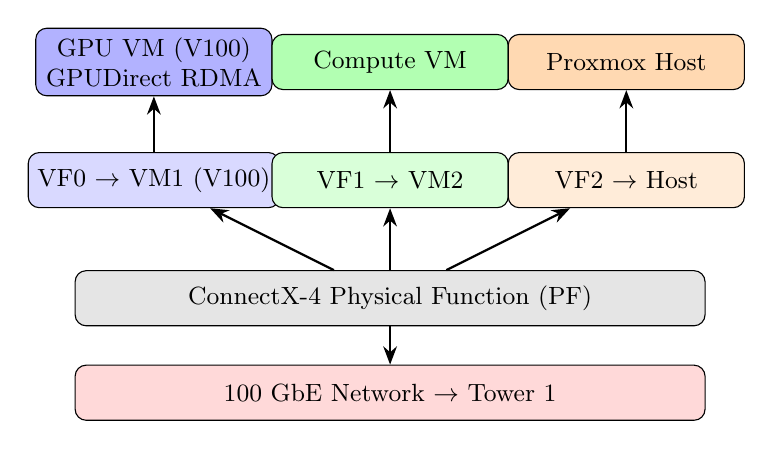
\begin{tikzpicture}[
    node distance=0.6cm,
    box/.style={rectangle, draw, rounded corners, minimum width=3cm, minimum height=0.7cm, align=center, font=\small},
    arrow/.style={->, thick, >=Stealth}
]
    % Physical NIC
    \node[box, fill=gray!20, minimum width=8cm] (pf) at (0,0) {ConnectX-4 Physical Function (PF)};

    % Virtual Functions
    \node[box, fill=blue!15] (vf0) at (-3,1.5) {VF0 $\to$ VM1 (V100)};
    \node[box, fill=green!15] (vf1) at (0,1.5) {VF1 $\to$ VM2};
    \node[box, fill=orange!15] (vf2) at (3,1.5) {VF2 $\to$ Host};

    % VMs
    \node[box, fill=blue!30] (vm1) at (-3,3) {GPU VM (V100)\\GPUDirect RDMA};
    \node[box, fill=green!30] (vm2) at (0,3) {Compute VM};
    \node[box, fill=orange!30] (host) at (3,3) {Proxmox Host};

    % Network
    \node[box, fill=red!15, minimum width=8cm] (net) at (0,-1.2) {100 GbE Network $\to$ Tower 1};

    \draw[arrow] (pf) -- (vf0);
    \draw[arrow] (pf) -- (vf1);
    \draw[arrow] (pf) -- (vf2);
    \draw[arrow] (vf0) -- (vm1);
    \draw[arrow] (vf1) -- (vm2);
    \draw[arrow] (vf2) -- (host);
    \draw[arrow] (pf) -- (net);
\end{tikzpicture}
\caption{SR-IOV architecture: ConnectX-4 presents multiple VFs, enabling the GPU VM to have dedicated RDMA access while other VMs share the physical NIC.}
\label{fig:sriov}
\end{figure}

\subsection{SR-IOV Setup on ConnectX-4}

The Mellanox ConnectX-4 supports up to 126 VFs per physical port. SR-IOV setup involves:

\begin{enumerate}[noitemsep]
    \item \textbf{Enable SR-IOV in BIOS}: Enable VT-d (Intel) or AMD-Vi, and enable SR-IOV in PCIe settings
    \item \textbf{Enable VFs on the NIC}: Write the desired VF count to the sysfs interface: \texttt{echo 4 > /sys/class/net/enp1s0f0/device/sriov\_numvfs}
    \item \textbf{Verify VF creation}: \texttt{ip link show enp1s0f0} should list VFs with MAC addresses
    \item \textbf{Pass VF to VM}: In Proxmox, add the VF's PCI address as a passthrough device to the GPU VM
    \item \textbf{Configure RDMA in VM}: Inside the VM, install rdma-core and OFED, then verify \texttt{ibv\_devinfo} shows the VF device
\end{enumerate}

\subsection{GPUDirect RDMA with SR-IOV}

For GPUDirect RDMA to work through an SR-IOV VF:

\begin{itemize}[noitemsep]
    \item The GPU and the NIC VF must be in the same IOMMU group or ACS must be relaxed
    \item The VM must have both the GPU and NIC VF passed through (not emulated)
    \item \texttt{nvidia-peermem} must be loaded inside the VM
    \item The hypervisor must not interpose on DMA between the GPU and NIC VF
\end{itemize}

\paragraph{IOMMU group challenge.}
On consumer motherboards, GPUs and NIC slots often land in different IOMMU groups, preventing peer-to-peer DMA. The ACS override patch (\texttt{pcie\_acs\_override=downstream,multifunction} kernel parameter) forces all devices into a single IOMMU group, enabling passthrough at the cost of reduced isolation. For a dedicated GPU compute VM, this tradeoff is acceptable.

\subsection{SR-IOV on Intel X710 and Aquantia AQC107}

\begin{table}[htbp]
\centering
\caption{SR-IOV support across lab NICs}
\label{tab:sriov-nics}
\begin{tabular}{@{}llccc@{}}
\toprule
\textbf{NIC} & \textbf{Node} & \textbf{SR-IOV} & \textbf{Max VFs} & \textbf{RDMA} \\
\midrule
Mellanox ConnectX-4 & Tower 1 \& 2 & Yes & 126 & Native RoCEv2 \\
Intel X710 10GbE & Cerberus & Yes & 64 & iWARP \\
Aquantia AQC107 10GbE & Chimera & No & 0 & None (SoftRoCE only) \\
\bottomrule
\end{tabular}
\end{table}

The Intel X710 supports SR-IOV with up to 64 VFs and native iWARP RDMA. However, iWARP has higher latency than RoCEv2 (${\sim}10~\mu$s vs.\ ${\sim}2~\mu$s) and is not supported by NVSHMEM. The Aquantia AQC107 lacks SR-IOV entirely, limiting Chimera to SoftRoCE on bare metal.

%=============================================================================
\section{Integration Plan: Kokkos Remote Spaces on Lab Cluster}
\label{sec:integration}
%=============================================================================

\subsection{Target Configuration}

\begin{table}[htbp]
\centering
\caption{Kokkos Remote Spaces deployment targets}
\label{tab:deployment}
\begin{tabular}{@{}lllll@{}}
\toprule
\textbf{Node} & \textbf{GPUs} & \textbf{NIC} & \textbf{Backend} & \textbf{GPUDirect} \\
\midrule
Tower 2 VM & 2$\times$ V100 & ConnectX-4 VF & NVSHMEM & Yes (BAR1=32GB) \\
Tower 1 & RTX 5070 Ti & ConnectX-4 & MPI one-sided & No (Windows) \\
Cerberus & 2$\times$ RTX 5090 & Intel X710 & MPI one-sided & Partial (ReBAR) \\
Chimera & 3$\times$ RTX 3090 & Aquantia AQC107 & MPI one-sided & Partial (ReBAR) \\
\bottomrule
\end{tabular}
\end{table}

The primary NVSHMEM + GPUDirect testing path is Tower~2 with the V100 GPUs and ConnectX-4 100~GbE. Consumer nodes fall back to the MPI one-sided backend with host-staged transfers.

\subsection{Build Plan}

The build process targets three configurations:

\begin{enumerate}[noitemsep]
    \item \textbf{NVSHMEM + CUDA (Tower 2)}: Install NVSHMEM 2.x, build Kokkos with \texttt{Kokkos\_ENABLE\_CUDA=ON}, build Kokkos Remote Spaces with \texttt{KRS\_ENABLE\_NVSHMEMSPACE=ON}. This enables GPU-initiated RDMA through ConnectX-4.

    \item \textbf{MPI one-sided + CUDA (Cerberus/Chimera)}: Build Kokkos with CUDA, build Kokkos Remote Spaces with \texttt{KRS\_ENABLE\_MPISPACE=ON}. Remote accesses use \texttt{MPI\_Put}/\texttt{MPI\_Get} through the host, with GPU data staged via \texttt{cudaMemcpy}.

    \item \textbf{MPI one-sided + Serial (Tower 1)}: CPU-only fallback for the Windows node. Uses OpenMPI for Windows or WSL2 with MPI.
\end{enumerate}

\subsection{Benchmark Plan}

\begin{table}[htbp]
\centering
\caption{Planned benchmark matrix}
\label{tab:benchmarks}
\begin{tabular}{@{}llll@{}}
\toprule
\textbf{Benchmark} & \textbf{Metric} & \textbf{NVSHMEM Path} & \textbf{MPI Path} \\
\midrule
\texttt{randomaccess} & GUPS & V100$\leftrightarrow$V100 & 3090$\leftrightarrow$5090 \\
\texttt{stream} & GB/s bandwidth & V100 (GPUDirect) & Host-staged \\
\texttt{access\_overhead} & Latency ($\mu$s) & GPU-initiated & CPU-initiated \\
\texttt{cgsolve} & Time-to-solution & Distributed V100 & Distributed 3090 \\
\bottomrule
\end{tabular}
\end{table}

The key comparison is NVSHMEM GPU-initiated RDMA (V100 + ConnectX-4, zero host involvement) vs.\ MPI host-staged RDMA (consumer GPU + SoftRoCE, CPU mediates every transfer). We expect $10\text{--}100\times$ latency advantage for the NVSHMEM path on fine-grained access patterns.

%=============================================================================
\section{UCX Toolkit: Transport Abstraction and Testing}
\label{sec:ucx}
%=============================================================================

UCX (Unified Communication X)~\cite{ucx} is an open-source communication framework developed by the UCF Consortium that provides a portable, high-performance transport layer for RDMA, shared memory, and TCP. UCX~v1.17.0 is installed on both cluster nodes at \texttt{/usr/local/ucx} and serves as the transport backend for OpenMPI, UCC, and NCCL on the lab cluster.

\subsection{UCX Architecture}

UCX is organized into four layers:

\begin{itemize}[noitemsep]
    \item \textbf{UCP (Protocol)}: High-level API for tag matching, RMA, atomic operations, and streaming. Applications typically program against UCP, which handles multi-rail selection, rendezvous protocol negotiation, and memory registration caching.
    \item \textbf{UCT (Transport)}: Low-level transport interface abstracting InfiniBand verbs (\texttt{rc}, \texttt{dc}, \texttt{ud}), RoCE, TCP, shared memory (\texttt{posix}, \texttt{sysv}, \texttt{cma}), and CUDA IPC/GDR transports. Each transport exposes bandwidth, latency, and capability metadata for automatic selection.
    \item \textbf{UCS (Services)}: Utility layer providing memory pools, async event handling, data structures, and architecture-specific optimizations.
    \item \textbf{UCM (Memory)}: Memory event hooks for tracking \texttt{mmap}/\texttt{munmap}/\texttt{cudaMalloc} to maintain registration cache coherency.
\end{itemize}

\subsection{Transport Selection for Lab Hardware}

UCX selects transports automatically based on available hardware, but the \texttt{UCX\_TLS} environment variable allows explicit control. The relevant transports for each cluster node are:

\begin{table}[htbp]
\centering
\caption{UCX transport availability by cluster node}
\label{tab:ucx-transports}
\begin{tabular}{@{}llll@{}}
\toprule
\textbf{Node} & \textbf{NIC Transport} & \textbf{GPU Transport} & \textbf{Intra-node} \\
\midrule
Tower 2 (V100) & \texttt{rc\_mlx5} (RoCEv2) & \texttt{cuda\_ipc}, \texttt{gdr\_copy} & \texttt{posix}, \texttt{cma} \\
Tower 1 (5070 Ti) & \texttt{rc\_mlx5} (RoCEv2) & \texttt{cuda\_copy} & \texttt{posix}, \texttt{cma} \\
Cerberus (5090) & \texttt{tcp} (X710) & \texttt{cuda\_copy} & \texttt{posix}, \texttt{cma} \\
Chimera (3090) & \texttt{tcp} (AQC107) & \texttt{cuda\_copy} & \texttt{posix}, \texttt{cma} \\
\bottomrule
\end{tabular}
\end{table}

Tower~2's ConnectX-4 enables \texttt{rc\_mlx5}---UCX's native InfiniBand Reliable Connection transport via the mlx5 driver, which bypasses the kernel and posts work requests directly to the NIC's send queue. The \texttt{gdr\_copy} transport uses GPUDirect RDMA for small messages ($<$8~KB) by mapping GPU BAR1 memory into the CPU address space for low-latency access. For consumer-NIC nodes (Cerberus, Chimera), UCX falls back to \texttt{tcp}, which provides correctness but not RDMA-level latency.

\subsection{UCX Performance Testing}

UCX ships with \texttt{ucx\_perftest}, a built-in benchmarking tool that measures point-to-point bandwidth and latency across all supported transports. The key test modes are:

\begin{table}[htbp]
\centering
\caption{UCX perftest configurations for the lab cluster}
\label{tab:ucx-perftests}
\begin{tabular}{@{}lllll@{}}
\toprule
\textbf{Test} & \textbf{Mode} & \textbf{Transport} & \textbf{Path} & \textbf{Measures} \\
\midrule
\texttt{tag\_bw} & UCP Tag & \texttt{rc\_mlx5} & Tower 2 $\leftrightarrow$ Tower 1 & Bandwidth (GB/s) \\
\texttt{tag\_lat} & UCP Tag & \texttt{rc\_mlx5} & Tower 2 $\leftrightarrow$ Tower 1 & Latency ($\mu$s) \\
\texttt{put\_bw} & UCT RMA & \texttt{rc\_mlx5} & Tower 2 $\leftrightarrow$ Tower 1 & One-sided BW \\
\texttt{tag\_bw} & UCP Tag & \texttt{tcp} & Cerberus $\leftrightarrow$ Chimera & TCP fallback BW \\
\texttt{tag\_bw} & UCP Tag & \texttt{cuda\_ipc} & V100$_0$ $\leftrightarrow$ V100$_1$ & Intra-node GPU \\
\bottomrule
\end{tabular}
\end{table}

The server-side command for ConnectX-4 bandwidth testing is \texttt{ucx\_perftest -t tag\_bw -d mlx5\_0 -m host}, and the client connects with \texttt{ucx\_perftest <server\_ip> -t tag\_bw -d mlx5\_0 -m host}. For CUDA-aware testing, the \texttt{-m cuda} flag allocates buffers via \texttt{cudaMalloc} and exercises the \texttt{gdr\_copy} or \texttt{cuda\_copy} transport paths.

\subsection{UCX with CUDA and GPUDirect}

When UCX detects CUDA-capable GPUs and the \texttt{nvidia-peermem} module is loaded, it enables two GPU-specific transports:

\begin{itemize}[noitemsep]
    \item \textbf{\texttt{gdr\_copy}}: Uses GPUDirect RDMA via BAR1 mapping for small messages. The CPU writes directly to GPU memory through the BAR1 aperture, achieving ${\sim}1~\mu$s latency for messages under 8~KB. Requires datacenter GPUs with large BAR1 (V100: 32~GB).
    \item \textbf{\texttt{cuda\_copy}}: Falls back to \texttt{cudaMemcpy} for host-staging. The transfer path is GPU~$\to$ Host Pinned Memory~$\to$ NIC~$\to$ Network. Adds ${\sim}5$--$10~\mu$s per hop but works on all CUDA GPUs regardless of BAR1 size.
    \item \textbf{\texttt{cuda\_ipc}}: For intra-node multi-GPU, uses CUDA IPC handles to map one GPU's memory into another GPU's address space via NVLink or PCIe peer access. Relevant for the dual-V100 configuration on Tower~2.
\end{itemize}

The environment variable \texttt{UCX\_CUDA\_COPY\_ASYNC\_MEM\_TYPE=cuda} enables asynchronous staging via CUDA streams, overlapping data movement with kernel execution. Combined with \texttt{UCX\_REG\_NONBLOCK\_MEM\_TYPES=cuda}, this avoids blocking on memory registration for dynamically allocated GPU buffers.

\subsection{UCX Integration with Kokkos Remote Spaces}

UCX serves as the transport layer when Kokkos Remote Spaces uses the MPI one-sided backend with OpenMPI. The integration path is:

\begin{center}
Kokkos View (remote access) $\to$ \texttt{MPI\_Put}/\texttt{MPI\_Get} $\to$ OpenMPI $\to$ UCX UCP $\to$ UCT (\texttt{rc\_mlx5} or \texttt{tcp})
\end{center}

Building OpenMPI with UCX support requires \texttt{--with-ucx=/usr/local/ucx} at configure time. Once built, OpenMPI automatically delegates all point-to-point and one-sided operations to UCX, benefiting from its multi-rail selection, registration cache, and protocol negotiation. The \texttt{UCX\_NET\_DEVICES} variable restricts UCX to a specific NIC (e.g., \texttt{mlx5\_0}) to prevent unintended fallback to slower interfaces.

\subsection{Known UCX Issues for Consumer Hardware}

Several upstream UCX issues affect deployment on the heterogeneous lab cluster:

\begin{enumerate}[noitemsep]
    \item \textbf{cudaMallocAsync IPC incompatibility} (GitHub \#7110): CUDA stream-ordered allocations via \texttt{cudaMallocAsync} produce memory handles that UCX's IPC transport cannot share between processes. The workaround is to use standard \texttt{cudaMalloc} for buffers that cross process boundaries.

    \item \textbf{Transport selection robustness} (GitHub \#9908): When multiple network interfaces are present (e.g., ConnectX-4 + onboard Ethernet), UCX may select a suboptimal transport or fail to fall back correctly. Setting \texttt{UCX\_NET\_DEVICES=mlx5\_0} explicitly avoids this.

    \item \textbf{Cross-NUMA GPU latency regression} (GitHub \#3249): When a GPU and NIC are on different NUMA nodes, UCX's \texttt{gdr\_copy} path may exhibit $2$--$3\times$ higher latency due to cross-socket PCIe traffic. On Tower~2, the V100 and ConnectX-4 should be verified to be in the same NUMA domain via \texttt{numactl --hardware} and \texttt{nvidia-smi topo -m}.
\end{enumerate}

%=============================================================================
\section{Relevance to Adaptive RDMA Middleware}
\label{sec:relevance}
%=============================================================================

Kokkos Remote Spaces provides a complementary programming model to the lock-free C++/Rust middleware being developed for this thesis:

\begin{itemize}[noitemsep]
    \item \textbf{PGAS vs.\ explicit RDMA}: Kokkos Remote Spaces abstracts remote access behind array indexing; our middleware uses explicit SPSC ring buffers and libibverbs. The PGAS model is simpler to program but offers less control over transfer batching and QP routing.

    \item \textbf{Hot/cold tensor mapping}: Our WFA classifier's hot/cold distinction maps to Kokkos Remote Spaces' choice between scalar access (fine-grained, for hot tensors) and \texttt{deep\_copy} (bulk, for cold tensors). The Lassen performance data confirms that fine-grained access across NVLink boundaries drops by $4\times$, validating the need for bulk transfer optimization.

    \item \textbf{GPUDirect as shared infrastructure}: Both approaches benefit from GPUDirect RDMA. The \texttt{nvidia-peermem} setup, BAR1 configuration, and IOMMU group management documented here apply equally to NVSHMEM-backed Kokkos views and to raw libibverbs operations in our SPSC ring buffer.

    \item \textbf{SR-IOV for multi-tenant GPU clusters}: The SR-IOV configuration enables multiple VMs to share RDMA NICs while maintaining GPUDirect paths---relevant for deploying the middleware in virtualized or cloud environments.

    \item \textbf{UCX as unified transport}: UCX provides a single API across InfiniBand verbs, RoCE, TCP, and shared memory, with automatic transport selection. The middleware can delegate transport negotiation to UCX rather than implementing per-NIC code paths, while retaining the option of raw libibverbs for latency-critical SPSC ring buffer operations where UCX's protocol overhead (${\sim}0.5~\mu$s per message) is unacceptable.
\end{itemize}

%=============================================================================
\section{Conclusions}
%=============================================================================

\begin{enumerate}[noitemsep]
    \item Kokkos Remote Spaces provides a PGAS abstraction over four backends (SHMEM, NVSHMEM, ROCSHMEM, MPI one-sided), enabling distributed GPU memory access with minimal code changes compared to explicit MPI.

    \item The NVSHMEM backend is the primary path for GPU-initiated RDMA on our V100 hardware. Consumer GPUs (RTX 3090, 5090) can use the MPI one-sided backend with host-staged transfers, or attempt GPUDirect via ReBAR.

    \item GPUDirect RDMA requires \texttt{nvidia-peermem}, adequate BAR1 size (32~GB on V100 vs.\ 256~MB default on consumer GPUs), and compatible IOMMU configuration. The V100 on Tower~2 with ConnectX-4 is the only configuration guaranteed to support full GPUDirect.

    \item SR-IOV on ConnectX-4 enables NIC sharing between Proxmox VMs while preserving RDMA capability. The Intel X710 (Cerberus) supports SR-IOV with iWARP but lacks NVSHMEM compatibility. The Aquantia AQC107 (Chimera) lacks SR-IOV entirely.

    \item The Kokkos Remote Spaces benchmarks (randomaccess, stream, cgsolve) provide a validation framework for comparing NVSHMEM GPU-initiated RDMA against MPI host-staged transfers on the heterogeneous cluster.

    \item UCX~v1.17.0 provides transport abstraction across the heterogeneous cluster: \texttt{rc\_mlx5} for ConnectX-4 nodes (kernel-bypass RDMA), \texttt{gdr\_copy} for V100 GPUDirect small-message access via BAR1, and \texttt{tcp} fallback for consumer-NIC nodes. UCX also serves as the transport backend for OpenMPI-based Kokkos Remote Spaces deployments, with \texttt{ucx\_perftest} providing per-transport bandwidth and latency benchmarking.
\end{enumerate}

\bibliography{update14}
\bibliographystyle{plainnat}

\end{document}
